\documentclass[12pt, titlepage]{article}
\newcommand{\famname}{CFS}
\usepackage{booktabs}
\usepackage{tabularx}
\usepackage{longtable}
\usepackage{graphicx}
\usepackage{hyperref}
\hypersetup{
    colorlinks,
    citecolor=black,
    filecolor=black,
    linkcolor=red,
    urlcolor=blue
}
\usepackage[round]{natbib}

%% Comments

\usepackage{color}

\newif\ifcomments\commentstrue

\ifcomments
\newcommand{\authornote}[3]{\textcolor{#1}{[#3 ---#2]}}
\newcommand{\todo}[1]{\textcolor{red}{[TODO: #1]}}
\else
\newcommand{\authornote}[3]{}
\newcommand{\todo}[1]{}
\fi

\newcommand{\wss}[1]{\authornote{blue}{SS}{#1}}
\newcommand{\an}[1]{\authornote{magenta}{Malavika}{#1}}


\begin{document}

\title{Test Report: Curve Fitting Software(CFS)} 
\author{Malavika Srinivasan}
\date{\today}
	
\maketitle

\pagenumbering{roman}

\section{Revision History}

\begin{tabularx}{\textwidth}{p{3cm}p{2cm}X}
\toprule {\bf Date} & {\bf Version} & {\bf Notes}\\
\midrule
Dec 24, 2018 & 1.0 & Final version by Malavika \\
\bottomrule
\end{tabularx}

~\newpage

\section{Symbols, Abbreviations and Acronyms}

\renewcommand{\arraystretch}{1.2}
\begin{tabular}{l l} 
  \toprule		
  \textbf{symbol} & \textbf{description}\\
  \midrule 
  T & Test\\
  \bottomrule
\end{tabular}\\
~\newline
Also see the table of symbols in CA at: 
\url{https://github.com/Malavika-Srinivasan/CAS741/tree/master/docs/SRS/CA.pdf}\\



\newpage

\tableofcontents

\listoftables %if appropriate

\listoffigures %if appropriate

\newpage

\pagenumbering{arabic}

This document represents the test report of the test cases presented in 
the System Verification and Validation plan of \famname{}.

\section{Functional Requirements Evaluation}

This section describes the summary of test results for the test cases 
which 
test the functional requirements of \famname{}. Thirty ($30$) test cases 
are 
presented in section 5.1 of the System VnV plan. The summary of the test 
results is shown below.
~\newline
~\newline
\begin{tabularx}{\textwidth}{p{4cm}p{4cm}}
	\toprule {\bf Test cases} & {\bf Relative error}\\
	\midrule
	T1 - T30 & $1 \times 10^{-1}$ \\
	\bottomrule
\end{tabularx}
~\newline
\noindent All the test cases passed and the code coverage was 100\%.



\section{Nonfunctional Requirements Evaluation}

\subsection{Correctness}

The file named ``test\_correctness.py'' presents the test cases chosen 
for parallel testing. Some of the modules such as Interpolation and 
Regression 
were tested against Python and Matlab. 

\subsubsection{Scope}

\begin{itemize}
	\item Most of the methods ($6$ out of $8$) are implemented by 
	\famname{}. 
	These methods are tested against Python libraries.
	\item The remaining methods are tested against Matlab.
\end{itemize}

\subsubsection{Test Results}

All the methods except Hermite cubic interpolation passed in parallel 
testing. 
For Hermite cubic interpolation, the coefficients from \famname{} and 
Matlab 
were different. The test case still fails. However, the fit does not seem 
to be 
affected. The plots below are based on the following data. \\

\noindent \textbf{Input:}\\
t = [1,2,4,5]\\
y = [2,1,4,3]\\

The plots from both the softwares look the same. 

\begin{figure}[h!]
	\begin{center}
		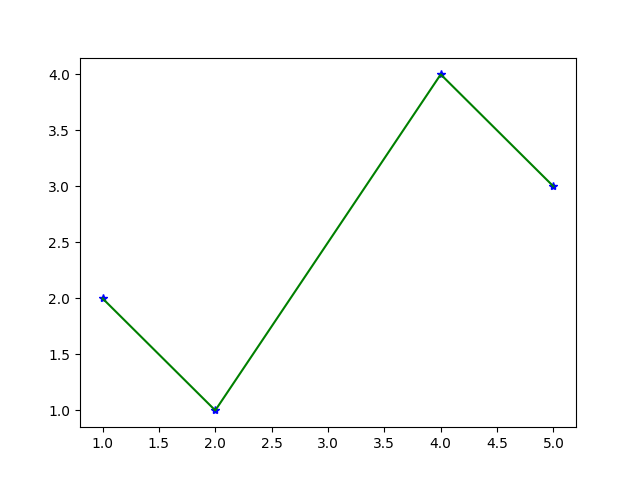
\includegraphics[width=0.6\textwidth]{PythonPlot.png}
		\caption{CFS Plot - Python wrapper}
		\label{Fig_Python} 
	\end{center}
\end{figure}

\begin{figure}[h!]
	\begin{center}
		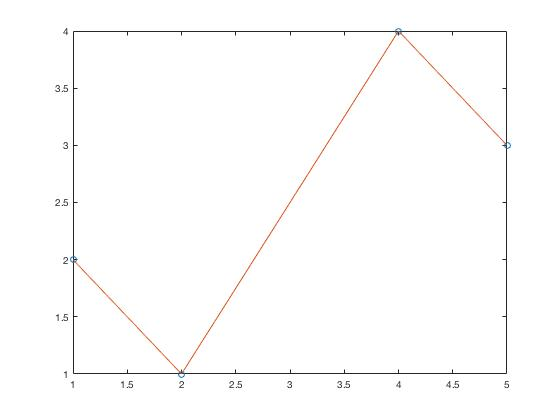
\includegraphics[width=0.6\textwidth]{Matlab.jpg}
		\caption{Matlab Plot}
		\label{Fig_Matlab} 
	\end{center}
\end{figure}

Both the solutions are acceptable.
		
\subsection{Portability}

\famname{} runs in windows and Unix. It was not tested in Linux due to 
lack of 
time and resources.

\subsection{Maintainability}

This test could not be conducted due to lack of resources. 
	
\section{Comparison to Existing Implementation}	

NA

\section{Unit Testing} Unit testing is conducted in Python.

\section{Changes Due to Testing} NA

\section{Automated Testing} All the test cases are automated except 
portability and parallel testing.
		
\section{Trace to Requirements} 


The following table (Table \ref{Table:Table_TraceabilityR}) shows the 
traceability mapping for test cases and the 
requirements. 

\begin{table} 
	\caption{\textbf{Requirements Traceability Matrix}}
	\label{Table:Table_TraceabilityR}  
	\begin{tabular}{|p{4cm}|p{4cm}|}
		\hline	
		\textbf{Test Number}  & \textbf{CA Requirements}\\
		\hline 
		T1(a,b)&   R1, R3       \\ \hline
		T2&  R1, R2       \\ \hline
		T3&   R1, R3       \\ \hline
		
		T4&  R4, R5, R6, R9, R10   \\ \hline
		T5&  R4, R5, R6, R9, R10   \\ \hline
		
		T6&  R4, R5, R6, R9, R10   \\ \hline
		T7&  R4, R5, R6, R9, R10   \\ \hline
		
		T8&  R4, R5, R6, R9, R10   \\ \hline
		T9&  R4, R5, R6, R9, R10   \\ \hline
		
		
		T10&  R4, R5, R7, R9, R10     \\ \hline
		T11&  R4, R5, R7, R9, R10     \\ \hline
		
		
		T12&  R4, R5, R7, R9, R10     \\ \hline
		
		
		T13&  R4, R8, R9, R10  \\ \hline
		T14&  R4, R8, R9, R10  \\ \hline
		T15&  R4, R8, R9, R10  \\ \hline
		
		
		T16&  R4, R8, R9, R10    \\ \hline
		T17& I R4, R8, R9, r10     \\ \hline
		
		T18&  R4, R8, R9, R10    \\ \hline
		T19&  R4, R8, R9, R10    \\ \hline
		
		T20&   R12\\ \hline
		T21&   R13\\ \hline
		T22&   R11\\ \hline
		
	\end{tabular}\\
\end{table}






		
\section{Trace to Modules}	

The following table (Table \ref{Table:Table_TraceabilityM}) shows the 
traceability mapping for test cases and the 
modules. All the modules except the ones listed as out of scope are 
covered and 
every access program in the module is tested. 

\begin{table}
	\caption{\textbf{Modules Traceability Matrix}}
	\label{Table:Table_TraceabilityM}  
	\begin{tabular}{|c|p{5cm}|}
		\hline	
		\textbf{Test Number} & \textbf{Modules} \\
		\hline 
		T1&  Input      \\ \hline
		T2&  Input      \\ \hline
		T3&  Input     \\ \hline
		T4&  Input     \\ \hline
		T5&  Interpolation      \\ \hline
		T6&  Interpolation     \\ \hline
		T7&  Interpolation     \\ \hline
		T8&  Interpolation      \\ \hline
		T9&  Interpolation     \\ \hline
		T10& Interpolation      \\ \hline
		T11& Interpolation      \\ \hline
		T12& Interpolation     \\ \hline
		T13& Interpolation     \\ \hline
		T14& Interpolation      \\ \hline
		T15& Regression     \\ \hline
		T16& Regression     \\ \hline
		T17& Regression      \\ \hline
		
	\end{tabular}\\
\end{table}


	

\section{Code Coverage Metrics} 

All the 3 modules mentioned in System VnV plan are tested. The code 
coverage 
metrics is 100\% in all the 3 modules. 

%\bibliographystyle{plainnat}

%\bibliography{SRS}

\end{document}